%%%%%%%%%%%%%%%%%%%%%%%%%%%%%%%%%%%%%%%%%
% Stylish Article
% LaTeX Template
% Version 2.0 (13/4/14)
%
% This template has been downloaded from:
% http://www.LaTeXTemplates.com
%
% Original author:
% Mathias Legrand (legrand.mathias@gmail.com)
%
% License:
% CC BY-NC-SA 3.0 (http://creativecommons.org/licenses/by-nc-sa/3.0/)
%
%%%%%%%%%%%%%%%%%%%%%%%%%%%%%%%%%%%%%%%%%

%----------------------------------------------------------------------------------------
%	PACKAGES AND OTHER DOCUMENT CONFIGURATIONS
%----------------------------------------------------------------------------------------

\documentclass[fleqn,10pt,onecolumn]{ipcc} % Document font size and equations flushed left

\usepackage{lipsum} % Required to insert dummy text. To be removed otherwise
\usepackage{tikz} % good quality graphs
\usepackage{pgfplots}
\usepackage[ampersand]{easylist}
\usetikzlibrary{pgfplots.groupplots}
\pgfplotsset{compat=newest}

%----------------------------------------------------------------------------------------
%	COLUMNS
%----------------------------------------------------------------------------------------

\setlength{\columnsep}{0.45cm} % Distance between the two columns of text
\setlength{\fboxrule}{0.75pt} % Width of the border around the abstract

%----------------------------------------------------------------------------------------
%	COLORS
%----------------------------------------------------------------------------------------

\definecolor{IrishGreen}{RGB}{0,0,90} % Color of the article title and sections
\definecolor{RoyalBlue}{RGB}{0,20,20} % Color of the boxes behind the abstract and headings

%----------------------------------------------------------------------------------------
%	HYPERLINKS
%----------------------------------------------------------------------------------------

\usepackage[colorlinks=true,bookmarks=true,plainpages=false,
linkcolor=IrishGreen, citecolor=IrishGreen, 
urlcolor=IrishGreen,pagebackref]{hyperref}%links in pdf
\usepackage[compress,numbers,comma]{natbib} %references
\usepackage{hypernat} %references
%----------------------------------------------------------------------------------------
%	ARTICLE INFORMATION
%----------------------------------------------------------------------------------------

\JournalInfo{OpenCL Notes} % Journal information
\Archive{} % Additional notes (e.g. copyright, DOI, review/research article)

\PaperTitle{OpenCL Notes} % Article title

\Authors{Christian Lalanne\textsuperscript{1}*, Adi\textsuperscript{1}, Rory\textsuperscript{2}} % Authors
\affiliation{\textsuperscript{1}\textit{Intel Parallel Computing Centre, Irish Centre for High End Computing}} % Author affiliation
\affiliation{\textsuperscript{2}\textit{Xilinx}} % Author affiliation
\affiliation{*\textbf{Corresponding author}: christian.lalanne@ichec.ie} % Corresponding author

\Keywords{OpenCL, GPU, Xeon Phi, Parallelism} % Keywords - if you don't want any simply remove all the text between the curly brackets
\newcommand{\keywordname}{Keywords} % Defines the keywords heading name

%----------------------------------------------------------------------------------------
%	ABSTRACT
%----------------------------------------------------------------------------------------

\Abstract{TBAL}

%----------------------------------------------------------------------------------------
\graphicspath{{figures/}}
%colours
\definecolor{IrishGreen}{cmyk}{0.70, 0.00, 0.80, 0.10}
\definecolor{RoyalBlue}{cmyk}{0.1, 0.0, 0.0, 0.02}

\begin{document}

\flushbottom % Makes all text pages the same height
\maketitle % Print the title and abstract box
\tableofcontents % Print the contents section
\listoffigures % list of figures
\thispagestyle{empty} % Removes page numbering from the first page

%----------------------------------------------------------------------------------------
%	ARTICLE CONTENTS
%----------------------------------------------------------------------------------------


\section*{Introduction} % The \section*{} command stops section numbering
\addcontentsline{toc}{section}{Introduction} % Adds this section to the table of contents with negative 
                                            %horizontal space equal to the indent for the numbered sections
\par{Molecular dynamics techniques grew rapidly in the last twenty years. 
The grow was fuelled by development of new scalable mathematical algorithms, availability 
of powerful hardware and better availability of ready to use software packages. DL\_POLY is one of 
these packages, widely adopted by the computational physics and material science communities.}
\par{DL\_POLY started its life in 1994 at Daresbury Laboratory, now part of Science \& Technology Facilities 
Council in United Kingdom. The main developers for the currect version are W Smith and IT Todorov. DL\_POLY is 
a general classical molecular dynamics code and was used to simulate macro molecules (both biological and synthetic),
complex fluids, materials and ionic liquids. DL\_POLY also plays an important role as sandbox for both development
of new methods and algorithms for molecular dynamics and testing of emerging hardware 
technologies\cite{dlpoly} and \cite{Todorov2006}.
The core code is written in Fortran 90 and optimised for distributed systems using domain decomposition, also OpenMP and CUDA ports exist as 
contributions to DL\_POLY but not part of the official distribution.
DL\_POLY is free of use for UK academics pursuing non-commerical research and available for licensing for the rest.
Over 3000 licenses were offered over the years worldwide.
}
\par{The Intel Xeon Phi co-processor is a novel accelerator technology that provides few appealing features as:
many cores, 60 cores with 240 hardware threads for the mid model, low power consumption, the same set as 
instructions as an Intel CPU, supports popular and standardised programming models as MPI and OpenMP and a 
theoretical peak of 1~TFlops.}
\par{In this communication we present the progress made in porting and optimising DL\_POLY to Xeon Phi co-processor. 
The rest of the paper is organised as follows: a short introduction to the methodology used for port and optimisation,
OpenMP implementation results in \sref{sec:openmp}, synchronous offload ones in \sref{sec:offload}, MPI symmetric
 running mode in \sref{sec:mpis}.}


%------------------------------------------------
\section{OpenCL}
\par{OpenCL(Open Computing Language) is an open standard for a low level(close to metal) api for parallel programming of 
    heterogeneous systems. Its usage spread through a wide range of platforms \emph{e.g. personal computers, servers and 
    embedded devices.}, and domains \emph{e.g. gaming and entertainment, scientific and medical software.}
    \cite{khronos,nvidia_opencl,opencl12}}

\par{OpenCL allow developers to execute computational kernels written with a subset of the C99 language(depending on the OpenCL 
    version) in different architectures \cite{nvidia_opencl} such as GPUs, CPUs, DSPs, FPGAs and other processors 
    \cite{wikipedia_opencl}. This kernels are executed in parallel in all these architectures, the parallel paradigms supported by
    OpenCL are data and task based parallel programming models\cite{opencl12}.}

\subsection{Important Concepts}
\par{...}

\subsection{Platform Model}
\par{\emph{Host} connected to one or more OpenCL \emph{devices}. One or more 
    \emph{compute units} belong to one OpenCL \emph{device}, and one \emph{compute unit} is divided into one or more
    \emph{processing elements}. The \emph{processing elements} in a \emph{compute unit} execute a single stream of instructions
    as SIMD units(execute in lockstep with a single stream of instructions) or SPMD units(each \emph{processing element} 
    maintains its own program counter), this model is shown in figure \ref{PlatformModel}\cite{opencl12}.}

\begin{figure}[!h]
    \centering
    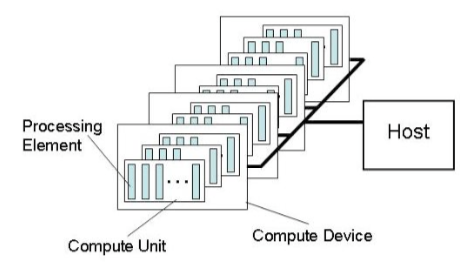
\includegraphics[width=0.4\textwidth]{figures/PlatformModel.png}
    \caption{Platform Model\cite{opencl12}.}
    \label{PlatformModel}
\end{figure}


\subsection{Memory Model}
\input{MemModel}
%------------------------------------------------
\section{OpenCL Mapping}
\par{This section will the most important features of the different architecture that we used for this work, it also explains the 
    mapping of the main OpenCL concepts into these different hardware architectures, also it will explain the most important 
    considerations of the OpenCL's \emph{kernel} execution into these devices}.

\subsection{CPU (Xeon)}
\label{sec:cpu}
\par{Table \ref{tab:xeon_arch} contains the main hardware characteristics of the Xeon CPU installed in fionn.}

\begin{table}[!h]
    \centering
    \begin{tabular}{| l | l | l | l |}
    \hline
    \# cores / socket& 10(out-of-order) \\ \hline
    \# threads / core& 2 \\ \hline
    \# sockets & 2 \\ \hline
    clock speed & 2.2 GHz \\ \hline
    typr & Ivy Bridge \\ \hline
    vector unit & 256-bit AVX \\ \hline
    L1 / core & 32KB(data)+32KB(instructions) 64KB total \\ \hline
    L2 / core & 256KB \\ \hline
    L3 /socket & 25MB \\ \hline
    \end{tabular}
    \caption{Xeon characteristics\cite{xeon_specs}.}
    \label{tab:xeon_arch}
\end{table}

\subsubsection{Mapping}

\par{The mapping of OpenCL concepts to Hardware are the same that in the Xeon Phi, see section \ref{sec:phi}.}

\par{{\color{red} PUT THE PICTURE OF THE OUTPUT OF DEVICEINFO AND PUT SOME COMMENTS ON IT!!!!!!}}

\subsection{Xeon Phi}
\subsubsection{Architecture}
\begin{itemize}
    \item 60 cores, In-order\cite{phi_specs}.
    \item 1.053 GHz of clock speed per core\cite{phi_specs}.
    \item Every core contains a 512-bit vector arithmetic unit(executing SIMD vector instructions). It fits 8 double precision 
        floating point numbers, or 16 single precision floating point numbers. Each core can issue a single vector instruction per
        cycle\cite{opencl_phi}(this execution looks similar to an Nvidia GPU \emph{warp}), so vector instructions issued by 
        different threads in the same core are sequentialized, they do not execute in parallel(at the same cycle).
    \item Each core has a L1 cache memory of 32KB for data and 32KB for instructions(64KB total). Miss latency 15-30
        cycles and access to L1 cache has a latency of 1 cycle\cite{opencl_phi}.
    \item Each core has a L2 cache of 512KB between data and instructions(combined 30MB of L2 cache). Miss latency 500-1000 cycles
        \cite{opencl_phi,phi_specs}.
    \item High speed interconect between L2 caches and the memory subsystem\cite{opencl_phi}.
    \item Simple automatic hardware prefetcher to L2\cite{opencl_phi}.
    \item Each core can execute 4 hardware threads simultaneously, 240 threads in total. These threads help to hide 
        instruction and memory latency\cite{opencl_phi}.
\end{itemize}

\par{OpenCL hides most of this detail from the programmer, figure \ref{PhiArch} shows a global view of the Intel Xeon Phi 
    architecture.\cite{opencl_phi}}

\begin{figure}[!h]
    \centering
    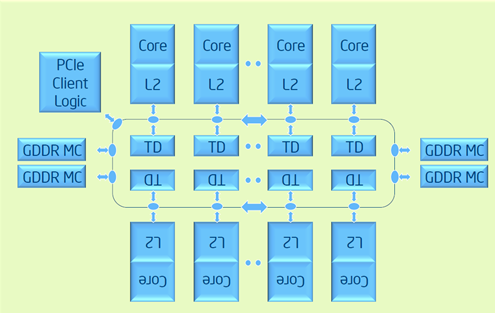
\includegraphics[width=0.6\textwidth]{figures/phi_arch.png}
    \caption{Intel Xeon Phi architecture\cite{opencl_phi}.}
    \label{PhiArch}
\end{figure}

\subsubsection{Mapping}
\begin{itemize}
    \item A \emph{work group} is the smallest task being scheduled on the threads\cite{opencl_phi}.
    \item \emph{Kernels} execute concurrently on multiple \emph{work items} in the SIMD units of every core\cite{opencl_phi_opt}.
    \item Each \emph{work group} is assigned to one thread that loops over all \emph{work items} within the \emph{work group} 
        with SIMD. So you have parallelism at the \emph{work group} level (vector instructions) and parallelism between 
        \emph{work groups} (threading)\cite{opencl_phi_opt}.
    \item At initialization time the Intel OpenCL driver creates 240 software threads and pins them to the hardware threads, then
        when you call \emph{clEnqueueNDRange()}, the intel driver schedules the \emph{work groups} of the current \emph{NDRange}
        into the 240 threads\cite{opencl_phi}.
    \item The OpenCL compiler implicitely vectorize the \emph{work group} routine based on dimension zero loop.
    \item The recommended work-group size for kernels is multiple of 16, which equals the SIMD width for the float and int data 
        type. The automatic vectorization module packs the work-items into SIMD packets of 16 items (for double as well), and 
        processed the rest (“tail”) of the work-group in a scalar way. In other words, a work-group with the size of 2*SIMD\_WIDTH 
        executes faster than, the one with the size of 2* SIMD\_WIDTH-1\cite{opencl_phi_opt,opencl_phi}.
    \item Non-uniform branching at dimension 0 the \emph{NDRange} is executed by flattening the code via predication and 
        ultimatelly executing both path of the branch and then apply masks, thus the usage of non-uniform branching is penalized by 
        a high overhead in the execution of the \emph{kernel}\cite{opencl_phi}.
    \item Using OpenCL \emph{local memory} does not provide any benefit on the Intel Xeon Phi. OpenCL \emph{local memory} is 
        allocated on the regular GDDR memory(\emph{global memory}) and is supported by the cache system like any other memory. 
        Therefore, it introduces additional overhead in terms of redundant data copy and management\cite{opencl_phi}.
    \item The combination of \emph{kernel} with barriers and \emph{work groups} nondivisible by 16, results in the execution of a
        scalar \emph{kernel}.
\end{itemize}

\begin{figure}[!h]
    \centering
    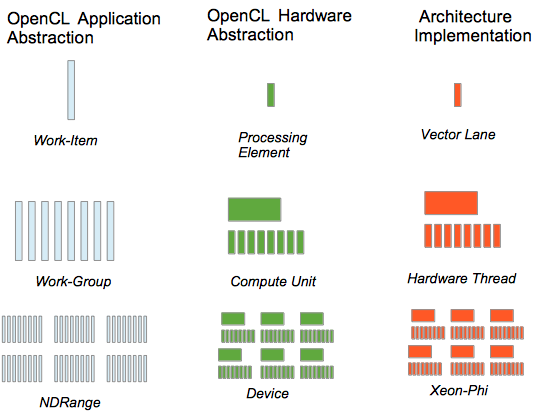
\includegraphics[width=0.7\textwidth]{figures/phi_model.png}
    \caption{OpenCL mapping for Intel Xeon Phi.}
    \label{PhiModel}
\end{figure}

\par{Figure \ref{PhiModel} shows a summary of the mapping of OpenCL concepts into the Intel Xeon Phi co-processor, figure 
    \ref{PhiDeviceInfo} shows the output of an OpenCL information request to the OpenCL run-time, it shows 236 
    \emph{compute units}(one per thread), the size of \emph{local memory} 32KB that match with the total amount of memory for L1 cache and
    the 6GB of total \emph{global memory} that matches with the amount of RAM available on the Intel Xeon Phi. In this context is 
    safe to assume that private memory on the Intel Xeon Phi is implemented via hardware registers.} 

\begin{figure}[!h]
    \centering
    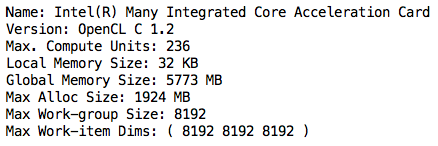
\includegraphics[width=0.7\textwidth]{figures/phi_device_info.png}
    \caption{Intel Xeon Phi device information.}
    \label{PhiDeviceInfo}
\end{figure}




\subsection{GPU}
\par{...}






\subsection{FPGA}
\par{...}


%------------------------------------------------
\section{Matrix Matrix Multiplication}
\par{To start this report we chose to analize the behaviour and performance of a Matrix Matrix multiplication algorithm 
    implementation, this is because this particular algorithm can be found in several scientific and HPC codes in several flavours
    and in its basic and more naive flavour is simple enough to be able to focus in OpenCL and the devices where is going to be 
    executed rather than the algorithm itself.}


\subsection{Naive}
\label{sec:naive}
\par{This implementation of this \emph{kernel} is as far as we know, the most 
    straightforward implementation of the matrix multiplication algorithm. 
    Optimisations were not implemented on this kernels as it can be seen in 
    listing \ref{naive_kernel}.} 
    
\par{Every instance of the \emph{kernel} calculates one element of the output 
    matrix(line 8), the \emph{NDRange} call is in 2 dimensions and all the 
    memory used for output and input data is global, this \emph{kernel}
    does not force caching or register usage via \emph{local} or \emph{private} 
    memory.}

\par{The results executing this kernel in different architectures with different 
    \emph{work group} dimensions can be seen in figure \ref{Naive}. From these 
    figures we can notice immediately that using dimensions greater than or 
    equal than 16 \emph{work items} in dimension 0 decreases the execution time 
    of the \emph{kernel} roughly 8 times in the case of Intel Xeon Phi. The
    Xeon CPU shows the same trend when the size of dimension 0 is greater or 
    equal than 2 but with an smaller decrease in execution time, 
    3.5 times approximately.}

\begin{figure}[!h]
    \centering
    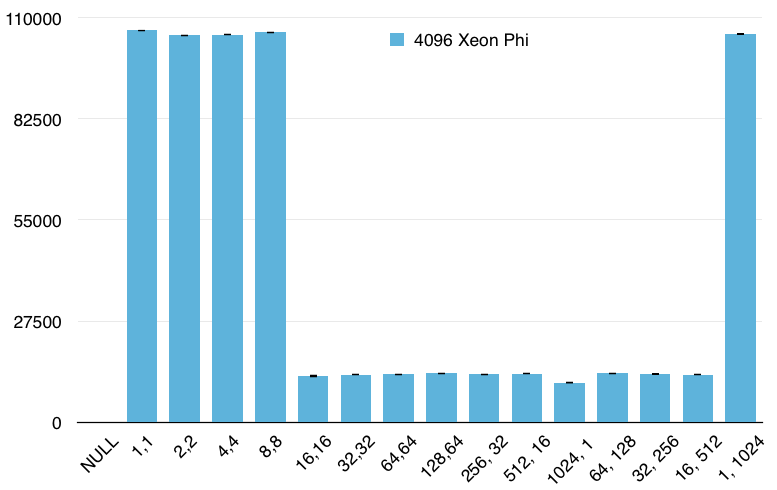
\includegraphics[width=0.49\textwidth]{figures/naive_phi.png}
    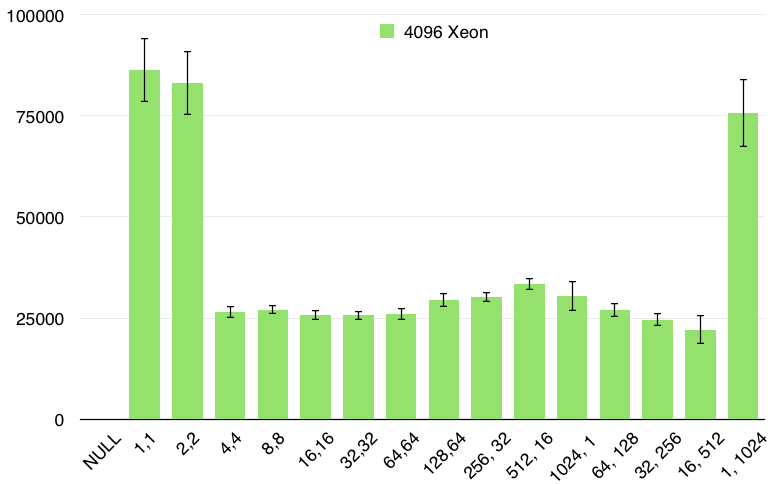
\includegraphics[width=0.49\textwidth]{figures/naive_cpu.png}
    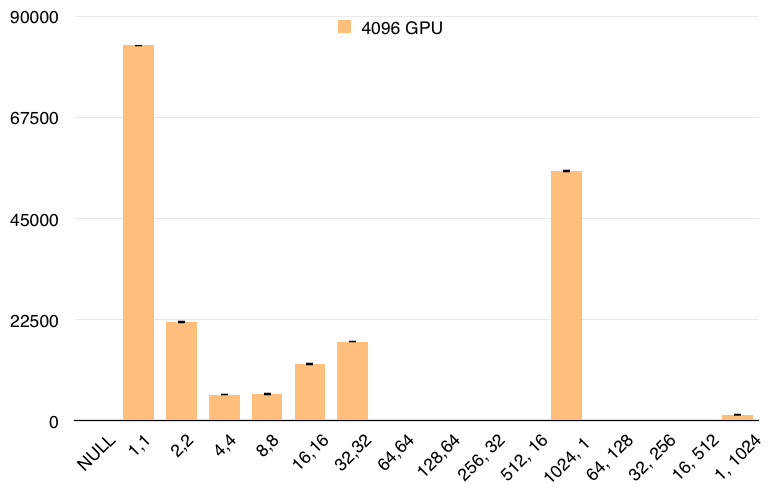
\includegraphics[width=0.49\textwidth]{figures/naive_gpu.png}
    \caption{Naive matrix multiplication results in different architectures.}
    \label{Naive}
\end{figure}

\par{Looking at listing \ref{llvm_code_naive_phi} we can realise that the 
    instructions that the Intel OpenCL compiler is generating are using a vector
    width of 16. This can explain the behaviour described previously and seen in
    figure \ref{Naive} for the Xeon Phi, being the \emph{work item} the basic 
    unit of computation in OpenCL, a \emph{work group} needs to have 16 \emph{
    work items} at least at dimension 0 to be able to use the entire width
    of the vector units available in the Xeon Phi. It seems that with numbers 
    less than 16 \emph{work items} inside of a \emph{work group} these 
    get serialized execution(using just one lane of the 16 available in the 
    vector registers of the Xeon Phi).}

\lstinputlisting[float,caption={Naive kernel LLVM code Intel Xeon Phi.}, 
    label={llvm_code_naive_phi}, 
    style=customc]
    {/Users/clalanne/GitHubProjects/OpenCLNotes/src/code/llvm_naive_phi.ll}

\par{Listing \ref{llvm_code_naive_cpu} and figure \ref{Naive} show the same 
    behaviour in the Xeon CPU, but with vector width of 4 instead of 16. Thus 
    in this case the Xeon CPU only needs 4 \emph{work items} at dimension 0
    of a \emph{work group} for the vectorization start to work. One intesting
    thing to notice is that the Xeon CPU has hardware support for AVX 
    vectorization, this means that the vector width should be of 256 bits, 
    available to fit 8 single precision numbers. We can se that even though 
    the Xeon CPU has support for AVX still the Intel OpenCL compiler generates
    by default instruction using just half of the vector width available.}

\lstinputlisting[float,caption={Naive kernel LLVM code Xeon.}, 
    label={llvm_code_naive_cpu}, 
    style=customc]
    {/Users/clalanne/GitHubProjects/OpenCLNotes/src/code/llvm_naive_cpu.ll}

\par{The way in which this \emph{kernel} is implemented, it shows poor data reuse
    forcing the system to request the data needed for computation from 
    \emph{global memory} using in a very inefficient way the cache system. 
    Figure \ref{vtune_naive} shows the profile of an execution of this \emph{
    kernel}, its possible to see the huge difference between the time that the
    \emph{kernel} spend bringing data from memory rather than using the data for
    computation(vgatherdps\footnote{Gather 2/4 packed 
    single-precision floating point values from memory referenced by the given 
    base address, dword indices and scale\cite{intrinsics}}
    \footnote{vgatherdps works by getting the data cache linewise per 
    invocation; this means that every time the gather instruction 
    is used, it will fetch only one cache line (CL), load all the values that 
    it is supposed to gather from it, store them in 
    the destination vector register, and finally zero out the bits of the 
    components that have been filled in the vector mask 
    register. As a consequence, the number of gather instruction depends on 
    the distribution of the data: 
    If all data resides in one CL then one gather instruction is sufficient; 
    in the worst case, each value is located in a different CL, 
    which will require sixteen gather instructions\cite{simd}.} vs vfmadd231ps).}

\begin{figure}[!h]
    \centering
    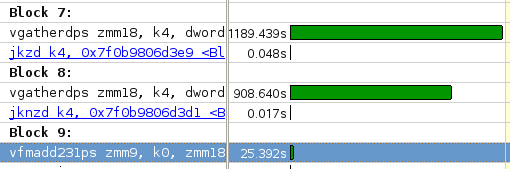
\includegraphics[width=0.49\textwidth]{figures/vtune_naive.png}
    \caption{Vtune profiler in the native kernel.}
    \label{vtune_naive}
\end{figure}

\par{{\color{red}Reading the listing \ref{naive_kernel}, its possible to see that there is no effort to use caches efficiently, the locality of
    memory access pattern its far from ideal. At the top of this, the gathering of data from memory results in having a high CPI(clock per
    instructions)\footnote{The CPI value of an application or function is an indication of how much latency affected its execution. 
    Higher CPI values mean there was more latency in your system – on average, it took more clockticks for an instruction to retire. 
    Latency in your system can be caused by cache misses, I/O, or other bottlenecks\cite{cpi}.} 
    rate poor vectorization and low L1 hit ratio for this kernel on the Xeon and Xeon Phi.}}

\par{For the GPU figure \ref{Naive} shows that not in all of the 
    \emph{work group} dimensions is possible to execute the kernel. 
    This is because the GPU run out of resources in those cases\cite{opencl_error},
    figure \ref{GpuDeviceInfo} and table \ref{tab:gpu_arch} show that the 
    maximum number of \emph{work group} size is of 1024 \emph{work items} which
    is exceeded by several of the \emph{work group} dimensions shown in figure 
    \ref{Naive}(\emph{e.g. 64x64}).}

\par{Figure \ref{NaiveRes} shows that GPUs achived the best performance in 
    comparison with the other architectures particularly
    in the case where the \emph{work group} dimension is 1x1024,
    this is mainly because the memory access patterns to access matrix A and B. 
    Access to matrix B its coalesced which means that the GPU can combine several 
    memory accesses into a single transaction, the memory access pattern for matrix 
    A also can be optimised, all the \emph{work items} in a warp access(read only)
    to the same memory space}.

\begin{figure}[!h]
    \centering
    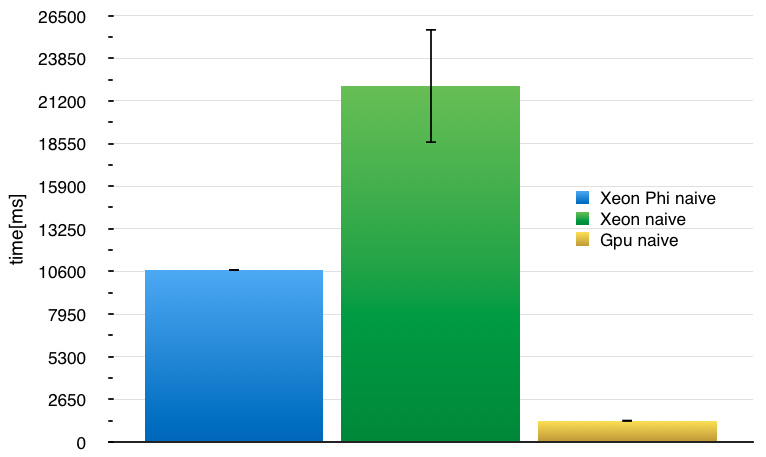
\includegraphics[width=0.49\textwidth]{figures/naiveRes.png}
    \caption{Comparison between the best cases in the different devices.}
    \label{NaiveRes}
\end{figure}

\par{Using warps and lock-step execution for the 
    GPU and vectorization of \emph{work items} for the Xeon and Xeon Phi, both
    memory access patterns are similar, with the difference that if we look at
    the GPU as a vector processor(warp execution) with double of the width that the
    Xeon Phi vector unit we can explain the better performance that this device 
    has against both Intel processors.}




\subsection{More Work}
\label{sec:moreWork}
\par{...\ref{MoreWork}\ref{MoreWorkComp}}

\begin{figure}[!h]
    \centering
    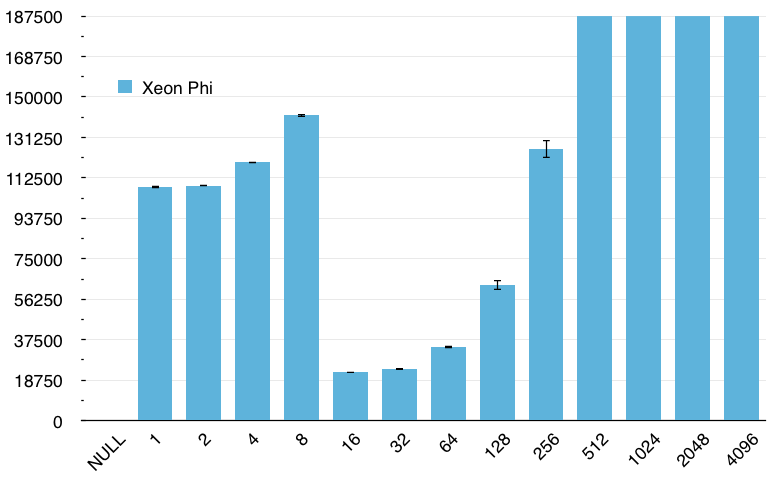
\includegraphics[width=0.49\textwidth]{figures/opt1_phi.png}
    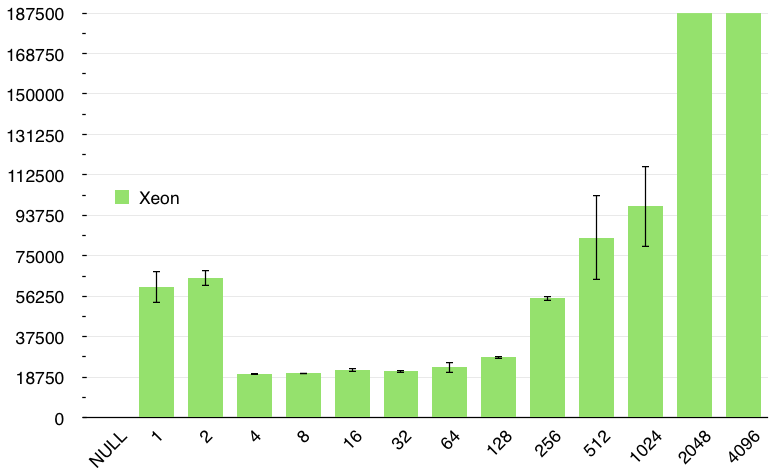
\includegraphics[width=0.49\textwidth]{figures/opt1_cpu.png}
    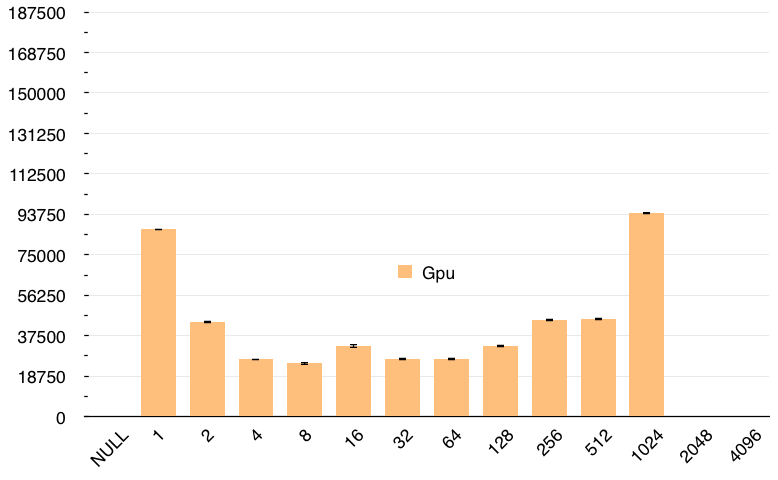
\includegraphics[width=0.49\textwidth]{figures/opt1_gpu.png}
    \caption{Matrix multiplication with more work in different architectures.}
    \label{MoreWork}
\end{figure}

\begin{figure}[!h]
    \centering
    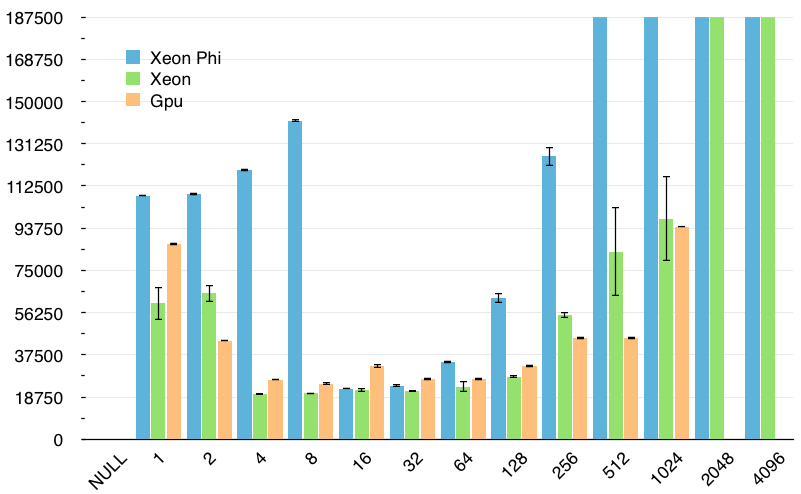
\includegraphics[width=0.6\textwidth]{figures/opt1_comp.png}
    \caption{Matrix multiplication with more work in different architectures comparison.}
    \label{MoreWorkComp}
\end{figure}


\subsection{Rows}
\label{sec:rows}
\par{...}

\subsection{Rows and Columns}
\label{sec:rowscols}

\par{Listing \ref{private_local_memory_kernel} shows the kernel that uses together \emph{private memory} to bring elements of A to 
    on-chip memory and \emph{local memory} to cache column B. In 
    this case the amount of \emph{local memory} to use is passed to the kernel as the fourth argument. The main idea for this is
    that all work items share the same column of B to avoid going into \emph{global memory}.}

\par{As in the previous kernel line \emph{12} shows the copy of elements to \emph{private memory} and line \emph{15} shows the 
    copy of elements from \emph{global memory} to \emph{local memory}, also ...\emph{expand on the use of barriers}.}

\lstinputlisting[float,caption={Kernel making use of \emph{private memory} and \emph{local memory}.},label={private_local_memory_kernel}, 
                style=customc]{/Users/clalanne/GitHubProjects/OpenCLNotes/src/code/private_local_memory.c}

\par{Figure \ref{RowsCols} shows the results of this kernel for different architectures, not all \emph{work group} dimensions 
    were possible to execute for this \emph{kernel}. For the case of the Xeon and Xeon Phi from the 32x32 the runtime returned
    error -5, that means was a failure to allocate resources\cite{opencl_error}, this mainly is because we are forcing to the 
    allocation of local memory ~16KB per \emph{work item}.

\begin{figure}[!h]
    \centering
    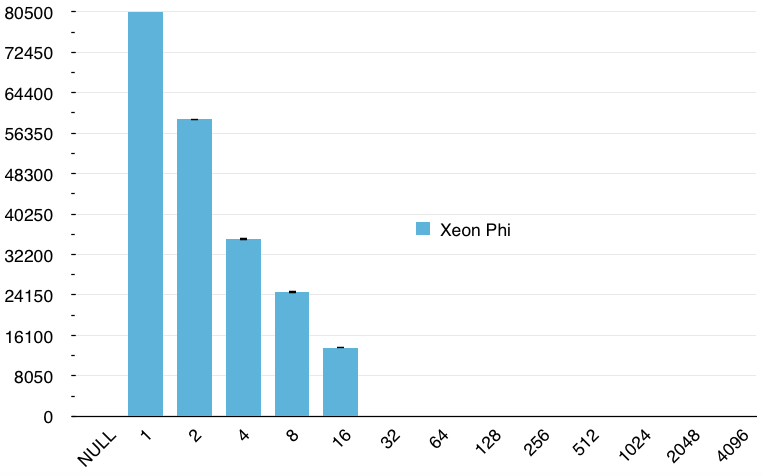
\includegraphics[width=0.49\textwidth]{figures/opt3_phi.png}
    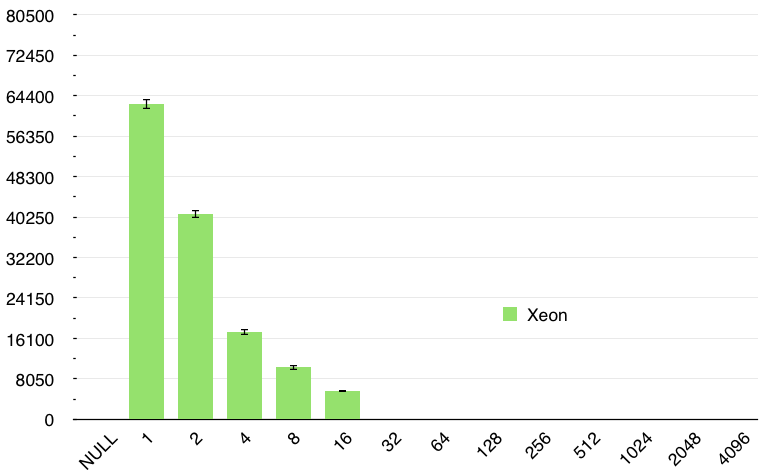
\includegraphics[width=0.49\textwidth]{figures/opt3_cpu.png}
    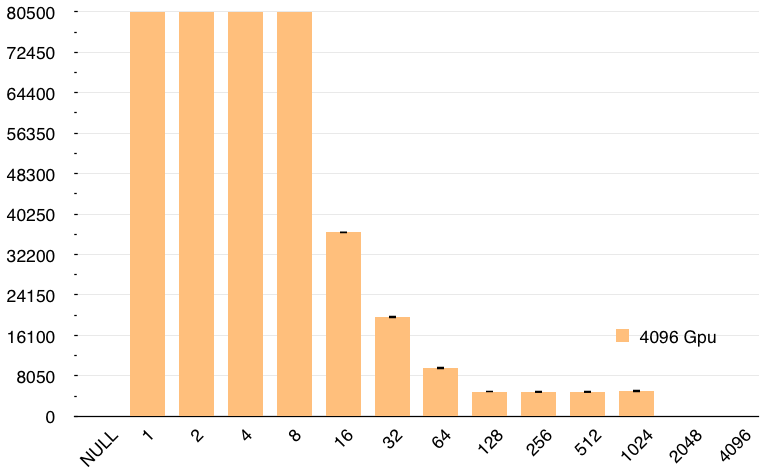
\includegraphics[width=0.49\textwidth]{figures/opt3_gpu.png}
    \caption{Rows and columns optimisation matrix multiplication in different architectures.}
    \label{RowsCols}
\end{figure}

\par{It seems to be a trade off here, between the the loop necesary to execute the copy of elements of B to \emph{local memory}
    (expensive gathering operations with a very poor L1 hit ratio) and the performance achieve in the loop where the kernel executes
    the computation(\emph{maybe vtune shot}).}

\par{In this case the best time is achived again by the GPU as we can see in figure \ref{RowsColsComp}, Also we can notice that the only 
    architectures that is able to take advantage of this optimisation is the Xeon. The Xeon Phi even have a warning in its 
    documentation about not using \emph{local} memory explicitelly as in this case, because of the cache system already is using 
    automatically this memory, and even warn about possible overhead time if this memory is defined explicitely\cite{opencl_phi}.}

\begin{figure}[!h]
    \centering
    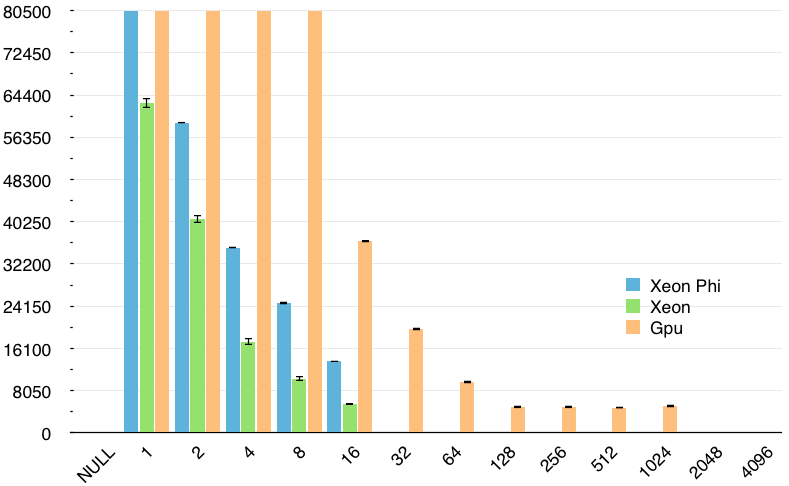
\includegraphics[width=0.6\textwidth]{figures/opt3_comp.png}
    \caption{Rows and columns optimisation matrix multiplication with more work in different architectures comparison.}
    \label{RowsColsComp}
\end{figure}


\subsection{Tiling}
\label{sec:tiling}
\par{...}

%------------------------------------------------
\section{Future Work and Conclusions}
\par{We successfully ported DL\_POLY to Xeon Phi and showed that without an intensive effort into optimisation it is 
difficult to fully take advantage of the Xeon Phi co-processor. Moderate success can be claimed for the OpenMP implementation were
we showed that for intensive routines with the right type of parallelism in native mode we can be as fast as the host, 
\emph{eg.} Shake. MPI symmetric seems to be a no go area as long as the homogenous decomposition of data is maintained.
By far the most promising is the offload mode, where synchronous offloading showed encouraging results. Future work will 
concentrate on mixing asynchronous computation and data transfers as promising sources of speed-up.}

%------------------------------------------------
\phantomsection
\section*{Acknowledgments} % The \section*{} command stops section numbering
\addcontentsline{toc}{section}{Acknowledgments} % Adds this section to the table of contents with 
                                                % negative horizontal space equal to the indent for the numbered sections
\par{to be added}


%----------------------------------------------------------------------------------------
%	REFERENCE LIST
%----------------------------------------------------------------------------------------
\phantomsection
%\nocite{*}
\bibliographystyle{unsrt}
\bibliography{report}

\phantomsection
\section*{Supplementary Information} % The \section*{} command stops section numbering
\addcontentsline{toc}{section}{Supplementary Information} % Adds this section to the table of contents with negative horizontal 
                                                        %space equal to the indent for the numbered sections
\par{...}

%----------------------------------------------------------------------------------------

\end{document}
